% Options for packages loaded elsewhere
\PassOptionsToPackage{unicode}{hyperref}
\PassOptionsToPackage{hyphens}{url}
\PassOptionsToPackage{dvipsnames,svgnames,x11names}{xcolor}
%
\documentclass[
  letterpaper,
  DIV=11,
  numbers=noendperiod,
  oneside]{scrartcl}

\usepackage{amsmath,amssymb}
\usepackage{lmodern}
\usepackage{iftex}
\ifPDFTeX
  \usepackage[T1]{fontenc}
  \usepackage[utf8]{inputenc}
  \usepackage{textcomp} % provide euro and other symbols
\else % if luatex or xetex
  \usepackage{unicode-math}
  \defaultfontfeatures{Scale=MatchLowercase}
  \defaultfontfeatures[\rmfamily]{Ligatures=TeX,Scale=1}
\fi
% Use upquote if available, for straight quotes in verbatim environments
\IfFileExists{upquote.sty}{\usepackage{upquote}}{}
\IfFileExists{microtype.sty}{% use microtype if available
  \usepackage[]{microtype}
  \UseMicrotypeSet[protrusion]{basicmath} % disable protrusion for tt fonts
}{}
\makeatletter
\@ifundefined{KOMAClassName}{% if non-KOMA class
  \IfFileExists{parskip.sty}{%
    \usepackage{parskip}
  }{% else
    \setlength{\parindent}{0pt}
    \setlength{\parskip}{6pt plus 2pt minus 1pt}}
}{% if KOMA class
  \KOMAoptions{parskip=half}}
\makeatother
\usepackage{xcolor}
\usepackage[left=1in,marginparwidth=2.0666666666667in,textwidth=4.1333333333333in,marginparsep=0.3in]{geometry}
\setlength{\emergencystretch}{3em} % prevent overfull lines
\setcounter{secnumdepth}{-\maxdimen} % remove section numbering
% Make \paragraph and \subparagraph free-standing
\ifx\paragraph\undefined\else
  \let\oldparagraph\paragraph
  \renewcommand{\paragraph}[1]{\oldparagraph{#1}\mbox{}}
\fi
\ifx\subparagraph\undefined\else
  \let\oldsubparagraph\subparagraph
  \renewcommand{\subparagraph}[1]{\oldsubparagraph{#1}\mbox{}}
\fi

\usepackage{color}
\usepackage{fancyvrb}
\newcommand{\VerbBar}{|}
\newcommand{\VERB}{\Verb[commandchars=\\\{\}]}
\DefineVerbatimEnvironment{Highlighting}{Verbatim}{commandchars=\\\{\}}
% Add ',fontsize=\small' for more characters per line
\usepackage{framed}
\definecolor{shadecolor}{RGB}{241,243,245}
\newenvironment{Shaded}{\begin{snugshade}}{\end{snugshade}}
\newcommand{\AlertTok}[1]{\textcolor[rgb]{0.68,0.00,0.00}{#1}}
\newcommand{\AnnotationTok}[1]{\textcolor[rgb]{0.37,0.37,0.37}{#1}}
\newcommand{\AttributeTok}[1]{\textcolor[rgb]{0.40,0.45,0.13}{#1}}
\newcommand{\BaseNTok}[1]{\textcolor[rgb]{0.68,0.00,0.00}{#1}}
\newcommand{\BuiltInTok}[1]{\textcolor[rgb]{0.00,0.23,0.31}{#1}}
\newcommand{\CharTok}[1]{\textcolor[rgb]{0.13,0.47,0.30}{#1}}
\newcommand{\CommentTok}[1]{\textcolor[rgb]{0.37,0.37,0.37}{#1}}
\newcommand{\CommentVarTok}[1]{\textcolor[rgb]{0.37,0.37,0.37}{\textit{#1}}}
\newcommand{\ConstantTok}[1]{\textcolor[rgb]{0.56,0.35,0.01}{#1}}
\newcommand{\ControlFlowTok}[1]{\textcolor[rgb]{0.00,0.23,0.31}{#1}}
\newcommand{\DataTypeTok}[1]{\textcolor[rgb]{0.68,0.00,0.00}{#1}}
\newcommand{\DecValTok}[1]{\textcolor[rgb]{0.68,0.00,0.00}{#1}}
\newcommand{\DocumentationTok}[1]{\textcolor[rgb]{0.37,0.37,0.37}{\textit{#1}}}
\newcommand{\ErrorTok}[1]{\textcolor[rgb]{0.68,0.00,0.00}{#1}}
\newcommand{\ExtensionTok}[1]{\textcolor[rgb]{0.00,0.23,0.31}{#1}}
\newcommand{\FloatTok}[1]{\textcolor[rgb]{0.68,0.00,0.00}{#1}}
\newcommand{\FunctionTok}[1]{\textcolor[rgb]{0.28,0.35,0.67}{#1}}
\newcommand{\ImportTok}[1]{\textcolor[rgb]{0.00,0.46,0.62}{#1}}
\newcommand{\InformationTok}[1]{\textcolor[rgb]{0.37,0.37,0.37}{#1}}
\newcommand{\KeywordTok}[1]{\textcolor[rgb]{0.00,0.23,0.31}{#1}}
\newcommand{\NormalTok}[1]{\textcolor[rgb]{0.00,0.23,0.31}{#1}}
\newcommand{\OperatorTok}[1]{\textcolor[rgb]{0.37,0.37,0.37}{#1}}
\newcommand{\OtherTok}[1]{\textcolor[rgb]{0.00,0.23,0.31}{#1}}
\newcommand{\PreprocessorTok}[1]{\textcolor[rgb]{0.68,0.00,0.00}{#1}}
\newcommand{\RegionMarkerTok}[1]{\textcolor[rgb]{0.00,0.23,0.31}{#1}}
\newcommand{\SpecialCharTok}[1]{\textcolor[rgb]{0.37,0.37,0.37}{#1}}
\newcommand{\SpecialStringTok}[1]{\textcolor[rgb]{0.13,0.47,0.30}{#1}}
\newcommand{\StringTok}[1]{\textcolor[rgb]{0.13,0.47,0.30}{#1}}
\newcommand{\VariableTok}[1]{\textcolor[rgb]{0.07,0.07,0.07}{#1}}
\newcommand{\VerbatimStringTok}[1]{\textcolor[rgb]{0.13,0.47,0.30}{#1}}
\newcommand{\WarningTok}[1]{\textcolor[rgb]{0.37,0.37,0.37}{\textit{#1}}}

\providecommand{\tightlist}{%
  \setlength{\itemsep}{0pt}\setlength{\parskip}{0pt}}\usepackage{longtable,booktabs,array}
\usepackage{calc} % for calculating minipage widths
% Correct order of tables after \paragraph or \subparagraph
\usepackage{etoolbox}
\makeatletter
\patchcmd\longtable{\par}{\if@noskipsec\mbox{}\fi\par}{}{}
\makeatother
% Allow footnotes in longtable head/foot
\IfFileExists{footnotehyper.sty}{\usepackage{footnotehyper}}{\usepackage{footnote}}
\makesavenoteenv{longtable}
\usepackage{graphicx}
\makeatletter
\def\maxwidth{\ifdim\Gin@nat@width>\linewidth\linewidth\else\Gin@nat@width\fi}
\def\maxheight{\ifdim\Gin@nat@height>\textheight\textheight\else\Gin@nat@height\fi}
\makeatother
% Scale images if necessary, so that they will not overflow the page
% margins by default, and it is still possible to overwrite the defaults
% using explicit options in \includegraphics[width, height, ...]{}
\setkeys{Gin}{width=\maxwidth,height=\maxheight,keepaspectratio}
% Set default figure placement to htbp
\makeatletter
\def\fps@figure{htbp}
\makeatother

\usepackage{booktabs}
\usepackage{longtable}
\usepackage{array}
\usepackage{multirow}
\usepackage{wrapfig}
\usepackage{float}
\usepackage{colortbl}
\usepackage{pdflscape}
\usepackage{tabu}
\usepackage{threeparttable}
\usepackage{threeparttablex}
\usepackage[normalem]{ulem}
\usepackage{makecell}
\usepackage{xcolor}
\KOMAoption{captions}{tableheading}
\makeatletter
\@ifpackageloaded{tcolorbox}{}{\usepackage[many]{tcolorbox}}
\@ifpackageloaded{fontawesome5}{}{\usepackage{fontawesome5}}
\definecolor{quarto-callout-color}{HTML}{909090}
\definecolor{quarto-callout-note-color}{HTML}{0758E5}
\definecolor{quarto-callout-important-color}{HTML}{CC1914}
\definecolor{quarto-callout-warning-color}{HTML}{EB9113}
\definecolor{quarto-callout-tip-color}{HTML}{00A047}
\definecolor{quarto-callout-caution-color}{HTML}{FC5300}
\definecolor{quarto-callout-color-frame}{HTML}{acacac}
\definecolor{quarto-callout-note-color-frame}{HTML}{4582ec}
\definecolor{quarto-callout-important-color-frame}{HTML}{d9534f}
\definecolor{quarto-callout-warning-color-frame}{HTML}{f0ad4e}
\definecolor{quarto-callout-tip-color-frame}{HTML}{02b875}
\definecolor{quarto-callout-caution-color-frame}{HTML}{fd7e14}
\makeatother
\makeatletter
\makeatother
\makeatletter
\makeatother
\makeatletter
\@ifpackageloaded{caption}{}{\usepackage{caption}}
\AtBeginDocument{%
\ifdefined\contentsname
  \renewcommand*\contentsname{Table of contents}
\else
  \newcommand\contentsname{Table of contents}
\fi
\ifdefined\listfigurename
  \renewcommand*\listfigurename{List of Figures}
\else
  \newcommand\listfigurename{List of Figures}
\fi
\ifdefined\listtablename
  \renewcommand*\listtablename{List of Tables}
\else
  \newcommand\listtablename{List of Tables}
\fi
\ifdefined\figurename
  \renewcommand*\figurename{Figure}
\else
  \newcommand\figurename{Figure}
\fi
\ifdefined\tablename
  \renewcommand*\tablename{Table}
\else
  \newcommand\tablename{Table}
\fi
}
\@ifpackageloaded{float}{}{\usepackage{float}}
\floatstyle{ruled}
\@ifundefined{c@chapter}{\newfloat{codelisting}{h}{lop}}{\newfloat{codelisting}{h}{lop}[chapter]}
\floatname{codelisting}{Listing}
\newcommand*\listoflistings{\listof{codelisting}{List of Listings}}
\makeatother
\makeatletter
\@ifpackageloaded{caption}{}{\usepackage{caption}}
\@ifpackageloaded{subcaption}{}{\usepackage{subcaption}}
\makeatother
\makeatletter
\@ifpackageloaded{tcolorbox}{}{\usepackage[many]{tcolorbox}}
\makeatother
\makeatletter
\@ifundefined{shadecolor}{\definecolor{shadecolor}{named}{true}}
\makeatother
\makeatletter
\@ifpackageloaded{sidenotes}{}{\usepackage{sidenotes}}
\@ifpackageloaded{marginnote}{}{\usepackage{marginnote}}
\makeatother
\makeatletter
\makeatother
\ifLuaTeX
  \usepackage{selnolig}  % disable illegal ligatures
\fi
\IfFileExists{bookmark.sty}{\usepackage{bookmark}}{\usepackage{hyperref}}
\IfFileExists{xurl.sty}{\usepackage{xurl}}{} % add URL line breaks if available
\urlstyle{same} % disable monospaced font for URLs
\hypersetup{
  pdftitle={How to Create Markov Model using R},
  pdfauthor={Astrid Yu, Ashley Leech},
  colorlinks=true,
  linkcolor={blue},
  filecolor={Maroon},
  citecolor={Blue},
  urlcolor={Blue},
  pdfcreator={LaTeX via pandoc}}

\title{How to Create Markov Model using R}
\author{Astrid Yu, Ashley Leech}
\date{2023-03-01}

\begin{document}
\maketitle
\ifdefined\Shaded\renewenvironment{Shaded}{\begin{tcolorbox}[frame hidden, colback={shadecolor}, boxrule=0pt, breakable, enhanced]}{\end{tcolorbox}}\fi

\renewcommand*\contentsname{Table of contents}
{
\hypersetup{linkcolor=}
\setcounter{tocdepth}{3}
\tableofcontents
}
\hypertarget{markov-in-class-exercise}{%
\section{Markov In-Class Exercise}\label{markov-in-class-exercise}}

We are tasked to examine the economic value of new treatments for a rare
type of cancer. The new treatments were designed to increase the health
of patients in remission \& to prevent them from relapsing back to
either Stage 1 or Stage 2.

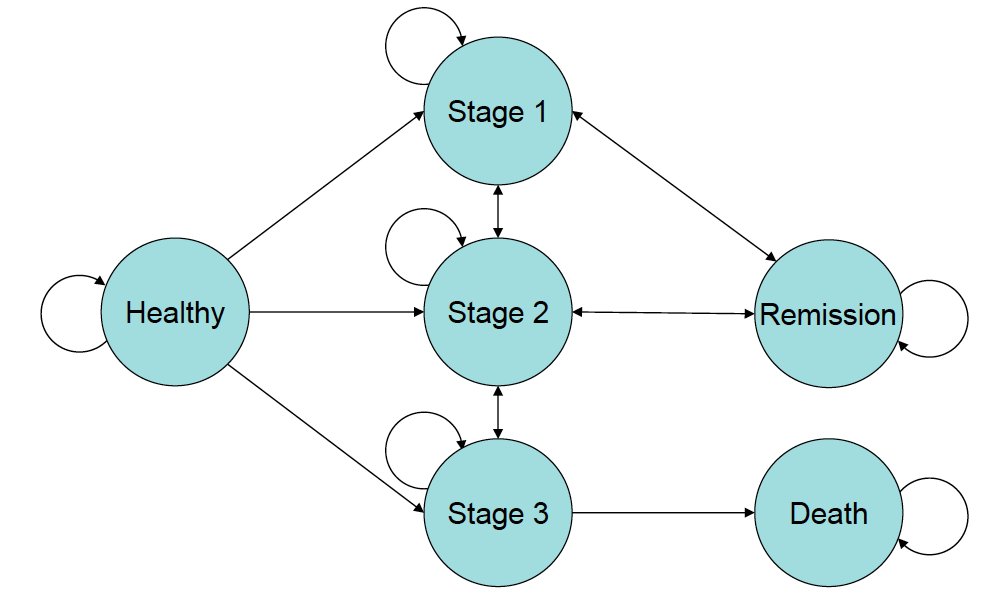
\includegraphics{exercise/markov_diagram.png}

Before the new drugs development, the transition probabilities were the
following:

\begin{longtable}[]{@{}
  >{\raggedright\arraybackslash}p{(\columnwidth - 2\tabcolsep) * \real{0.8488}}
  >{\raggedright\arraybackslash}p{(\columnwidth - 2\tabcolsep) * \real{0.1512}}@{}}
\toprule()
\begin{minipage}[b]{\linewidth}\raggedright
Description
\end{minipage} & \begin{minipage}[b]{\linewidth}\raggedright
Probability
\end{minipage} \\
\midrule()
\endhead
Probability of transition from Healthy to Stage 1 & 5\% \\
Probability of transition from Healthy to Stage 2 & 2\% \\
Probability of transition from Healthy to Stage 3 & 1\% \\
Probability of transition from Stage 1 to Stage 2 & 10\% \\
Probability of transition from Stage 1 to Remission & 25\% \\
Probability of transition from Stage 2 to Stage 1 & 5\% \\
Probability of transition from Stage 2 to Stage 3 & 15\% \\
Probability of transition from Stage 2 to Remission & 20\% \\
Probability of transition from Stage 3 to Stage 2 & 5\% \\
Probability of transition from Stage 3 to Death & 45\% \\
Probability of transition from Remission to Stage 1 & 10\% \\
Probability of transition from Remission to Stage 2 & 5\% \\
Probability of transition from Remission to Stage 1 when on Treatment A
& 10\% \\
Probability of transition from Remission to Stage 2 when on Treatment A
& 5\% \\
Probability of transition from Remission to Stage 1 when on Treatment B
& 8\% \\
Probability of transition from Remission to Stage 2 when on Treatment B
& 3\% \\
Probability of transition from Remission to Stage 1 when on Treatment C
& 5\% \\
Probability of transition from Remission to Stage 2 when on Treatment C
& 2\% \\
\bottomrule()
\end{longtable}

Each health state is associated with the following utilities:

\begin{longtable}[]{@{}ll@{}}
\toprule()
Description & Utility \\
\midrule()
\endhead
Utility of Healthy per cycle & 1 \\
Utility of Stage 1 per cycle & 0.88 \\
Utility of Stage 2 per cycle & 0.71 \\
Utility of Stage 3 per cycle & 0.36 \\
Utility of Remission per cycle & 0.95 \\
\bottomrule()
\end{longtable}

Patients in certain health states have to take medications and visit
their treating physician on a regular basis:

\begin{longtable}[]{@{}ll@{}}
\toprule()
Description & Costs / Other \\
\midrule()
\endhead
Number of visits per cycle in Stage 1 & 4 \\
Number of visits per cycle in Stage 2 & 12 \\
Number of visits per cycle in Stage 3 & 52 \\
Number of visits per cycle in Remission & 1 \\
Cost of a visit & \$ 100 \\
Cost of treatment per cycle in Stage 1 & \$ 1,200 \\
Cost of treatment per cycle in Stage 2 & \$ 6,000 \\
Cost of treatment per cycle in Stage 3 & \$ 18,000 \\
Cost of status quo per cycle in Remission & \$ 400 \\
Cost of Treatment A per cycle in Remission & \$ 10,000 \\
Cost of Treatment B per cycle in Remission & \$ 7,500 \\
Cost of Treatment C per cycle in Remission & \$ 12,500 \\
\bottomrule()
\end{longtable}

Assume an annual discount rate of 3\% and a 30-year time horizon.

\begin{tcolorbox}[enhanced jigsaw, rightrule=.15mm, toprule=.15mm, opacitybacktitle=0.6, colback=white, leftrule=.75mm, opacityback=0, bottomtitle=1mm, arc=.35mm, titlerule=0mm, colbacktitle=quarto-callout-note-color!10!white, breakable, title=\textcolor{quarto-callout-note-color}{\faInfo}\hspace{0.5em}{Note}, toptitle=1mm, bottomrule=.15mm, left=2mm, colframe=quarto-callout-note-color-frame, coltitle=black]

\textbf{What You Need to Prepare:}

\begin{enumerate}
\def\labelenumi{\arabic{enumi}.}
\tightlist
\item
  the Exercise excel file: we have the initial values for all the
  parameters and the procedures displayed in the excel formula.
\item
  the Function R file: it includes some advanced and long functions for
  the process. Lots of the functions are included in the \emph{dampack}
  R package.
\item
  R Studio or R. -- I highly recommende you to use R Studio
\end{enumerate}

\end{tcolorbox}

\hypertarget{step-1-parameterize-the-model}{%
\section{Step 1: Parameterize the
Model}\label{step-1-parameterize-the-model}}

Here we use the excel to upload all the parameters provided in the
excel.

Another ways is to define the parameters directly in the R.

We get a list of parameters named \emph{param\_sc}.

\begin{tabular}{l|l}
\hline
type & prefix\\
\hline
Probability & p\_\\
\hline
Rate & r\_\\
\hline
Matrix & m\_\\
\hline
Cost & c\_\\
\hline
Utility & u\_\\
\hline
Hazard Ratio & hr\_\\
\hline
\end{tabular}

\begin{Shaded}
\begin{Highlighting}[]
\NormalTok{input\_file }\OtherTok{=} \FunctionTok{normalizePath}\NormalTok{(}\FunctionTok{here}\NormalTok{(}\StringTok{"exercise/markov\_exercise.xlsx"}\NormalTok{))}
\NormalTok{input\_raw }\OtherTok{=}\NormalTok{ readxl}\SpecialCharTok{::}\FunctionTok{read\_xlsx}\NormalTok{(input\_file,}\AttributeTok{sheet=}\StringTok{"Parameters"}\NormalTok{)[,}\DecValTok{1}\SpecialCharTok{:}\DecValTok{7}\NormalTok{]}
\NormalTok{params\_sc }\OtherTok{=}\NormalTok{ input\_raw }\SpecialCharTok{\%\textgreater{}\%} 
  \FunctionTok{select}\NormalTok{(}\StringTok{\textasciigrave{}}\AttributeTok{Variable name}\StringTok{\textasciigrave{}}\NormalTok{, Value) }\SpecialCharTok{\%\textgreater{}\%}
  \FunctionTok{na.omit}\NormalTok{() }\SpecialCharTok{\%\textgreater{}\%}
  \FunctionTok{deframe}\NormalTok{() }\SpecialCharTok{\%\textgreater{}\%}
  \FunctionTok{as.list}\NormalTok{()}
\CommentTok{\# list2env(params\_sc, envir=.GlobalEnv)}

\NormalTok{v\_names\_states }\OtherTok{=} \FunctionTok{str\_sub}\NormalTok{(}\FunctionTok{names}\NormalTok{(}\FunctionTok{as\_tibble}\NormalTok{(params\_sc) }\SpecialCharTok{\%\textgreater{}\%} \FunctionTok{select}\NormalTok{(}\FunctionTok{starts\_with}\NormalTok{(}\StringTok{"u"}\NormalTok{))), }\DecValTok{2}\NormalTok{, }\SpecialCharTok{{-}}\DecValTok{1}\NormalTok{)}
\NormalTok{v\_n\_states }\OtherTok{\textless{}{-}} \FunctionTok{length}\NormalTok{(v\_names\_states)}
\NormalTok{v\_names\_str }\OtherTok{=} \FunctionTok{c}\NormalTok{(}\StringTok{"quo"}\NormalTok{, }\FunctionTok{str\_c}\NormalTok{(}\StringTok{"t"}\NormalTok{,}\FunctionTok{str\_sub}\NormalTok{(}\FunctionTok{names}\NormalTok{(}\FunctionTok{as\_tibble}\NormalTok{(params\_sc) }\SpecialCharTok{\%\textgreater{}\%} \FunctionTok{select}\NormalTok{(}\FunctionTok{starts\_with}\NormalTok{(}\StringTok{"cTrt"}\NormalTok{))), }\DecValTok{3}\NormalTok{, }\SpecialCharTok{{-}}\DecValTok{1}\NormalTok{)))}
\NormalTok{n\_strategies }\OtherTok{\textless{}{-}} \FunctionTok{length}\NormalTok{(v\_names\_str)}

\FunctionTok{options}\NormalTok{(}\StringTok{"scipen"}\OtherTok{=}\DecValTok{1000}\NormalTok{, }\StringTok{"digits"}\OtherTok{=}\DecValTok{2}\NormalTok{)}

\FunctionTok{t}\NormalTok{(}\FunctionTok{as\_tibble}\NormalTok{(params\_sc)) }\SpecialCharTok{\%\textgreater{}\%}
  \FunctionTok{kable}\NormalTok{(}\AttributeTok{caption =} \StringTok{"input params from excel"}\NormalTok{) }\SpecialCharTok{\%\textgreater{}\%}
  \FunctionTok{kable\_styling}\NormalTok{() }\SpecialCharTok{\%\textgreater{}\%}
  \FunctionTok{scroll\_box}\NormalTok{(}\AttributeTok{height =} \StringTok{"400px"}\NormalTok{)}
\end{Highlighting}
\end{Shaded}

\begin{table}

\caption{input params from excel}
\centering
\begin{tabular}[t]{l|r}
\hline
nPop & 1000.00\\
\hline
n\_cycles & 30.00\\
\hline
cycle\_length & 1.00\\
\hline
wtp & 5200.00\\
\hline
discount\_rate & 0.03\\
\hline
pHealthyStage1 & 0.05\\
\hline
pHealthyStage2 & 0.02\\
\hline
pHealthyStage3 & 0.01\\
\hline
pStage1Stage2 & 0.10\\
\hline
pStage1Remission & 0.25\\
\hline
pStage2Stage1 & 0.05\\
\hline
pStage2Stage3 & 0.15\\
\hline
pStage2Remission & 0.20\\
\hline
pStage3Stage2 & 0.05\\
\hline
pStage3Death & 0.45\\
\hline
pRemissionStage1 & 0.10\\
\hline
pRemissionStage2 & 0.05\\
\hline
pRemissionStage1\_trtA & 0.02\\
\hline
pRemissionStage2\_trtA & 0.01\\
\hline
pRemissionStage1\_trtB & 0.08\\
\hline
pRemissionStage2\_trtB & 0.03\\
\hline
pRemissionStage1\_trtC & 0.05\\
\hline
pRemissionStage2\_trtC & 0.02\\
\hline
rHealthyStage1 & 0.05\\
\hline
rHealthyStage2 & 0.02\\
\hline
rHealthyStage3 & 0.01\\
\hline
rStage1Stage2 & 0.12\\
\hline
rStage1Remission & 0.31\\
\hline
rStage2Stage1 & 0.06\\
\hline
rStage2Stage3 & 0.19\\
\hline
rStage2Remission & 0.26\\
\hline
rStage3Stage2 & 0.07\\
\hline
rStage3Death & 0.62\\
\hline
rRemissionStage1 & 0.11\\
\hline
rRemissionStage2 & 0.05\\
\hline
hrRemissionStage1\_trtA & 0.19\\
\hline
hrRemissionStage2\_trtA & 0.19\\
\hline
hrRemissionStage1\_trtB & 0.78\\
\hline
hrRemissionStage2\_trtB & 0.59\\
\hline
hrRemissionStage1\_trtC & 0.48\\
\hline
hrRemissionStage2\_trtC & 0.38\\
\hline
nVisitsStage1 & 4.00\\
\hline
nVisitsStage2 & 12.00\\
\hline
nVisitsStage3 & 52.00\\
\hline
nVisitsRemission & 1.00\\
\hline
cVisit & 100.00\\
\hline
cTreatmentStage1 & 1200.00\\
\hline
cTreatmentStage2 & 6000.00\\
\hline
cTreatmentStage3 & 18000.00\\
\hline
cTreatmentRemission & 400.00\\
\hline
cTrtA & 10000.00\\
\hline
cTrtB & 7500.00\\
\hline
cTrtC & 12500.00\\
\hline
uHealthy & 1.00\\
\hline
uStage1 & 0.88\\
\hline
uStage2 & 0.71\\
\hline
uStage3 & 0.36\\
\hline
uRemission & 0.95\\
\hline
uDeath & 0.00\\
\hline
\end{tabular}
\end{table}

\hypertarget{step-2-matrices}{%
\section{Step 2: Matrices}\label{step-2-matrices}}

With all the probabilities for transitions among all the stages, we'd
like to build a transition probability matrix which would contribute to
building Markov model traces later.

However, we might not have all the probabilities at the beginning. We
also mention how to change rates into probabilities here.

\hypertarget{if-all-probabilities-known-no-rate-to-probabilities-transitions}{%
\subsection{If All Probabilities Known (No Rate-to-Probabilities
Transitions)}\label{if-all-probabilities-known-no-rate-to-probabilities-transitions}}

\begin{Shaded}
\begin{Highlighting}[]
\NormalTok{build\_matrices }\OtherTok{\textless{}{-}} \ControlFlowTok{function}\NormalTok{(params, mtype) \{}
\NormalTok{  m\_X }\OtherTok{=} \FunctionTok{list}\NormalTok{()}
  \ControlFlowTok{for}\NormalTok{ (m }\ControlFlowTok{in}\NormalTok{ v\_names\_str)\{}
\NormalTok{    m\_X\_ }\OtherTok{=} \FunctionTok{matrix}\NormalTok{(}\DecValTok{0}\NormalTok{, }\AttributeTok{nrow =}\NormalTok{ v\_n\_states, }\AttributeTok{ncol =}\NormalTok{ v\_n\_states, }\AttributeTok{dimnames =} \FunctionTok{list}\NormalTok{(v\_names\_states,v\_names\_states))}
    \ControlFlowTok{for}\NormalTok{ (i }\ControlFlowTok{in} \FunctionTok{rownames}\NormalTok{(m\_X\_)) \{}
      \ControlFlowTok{for}\NormalTok{ (j }\ControlFlowTok{in} \FunctionTok{colnames}\NormalTok{(m\_X\_)) \{}
        \ControlFlowTok{if}\NormalTok{ (}\FunctionTok{paste0}\NormalTok{(mtype,i,j) }\SpecialCharTok{\%in\%} \FunctionTok{names}\NormalTok{(params)) \{}
\NormalTok{          m\_X\_[i,j] }\OtherTok{=} \FunctionTok{as.numeric}\NormalTok{(params[}\FunctionTok{paste0}\NormalTok{(mtype,i,j)])}
\NormalTok{        \}}
\NormalTok{      \}}
\NormalTok{    \}}
    
    \ControlFlowTok{if}\NormalTok{ (mtype }\SpecialCharTok{==} \StringTok{"p"}\NormalTok{) \{}
      \DocumentationTok{\#\# if drawing the probabilities from the given parameters and building a probability matrix}
      
      \ControlFlowTok{if}\NormalTok{ (}\FunctionTok{paste0}\NormalTok{(}\StringTok{"pRemissionStage1\_"}\NormalTok{,m) }\SpecialCharTok{\%in\%} \FunctionTok{names}\NormalTok{(params)) \{}
        \DocumentationTok{\#\# the relapse probs change over the strategies. A special rule here. }
\NormalTok{        m\_X\_[}\StringTok{"Remission"}\NormalTok{,}\StringTok{"Stage1"}\NormalTok{] }\OtherTok{=} \FunctionTok{as.numeric}\NormalTok{(params[}\FunctionTok{paste0}\NormalTok{(}\StringTok{"pRemissionStage1\_"}\NormalTok{,m)])}
\NormalTok{        m\_X\_[}\StringTok{"Remission"}\NormalTok{,}\StringTok{"Stage2"}\NormalTok{] }\OtherTok{=} \FunctionTok{as.numeric}\NormalTok{(params[}\FunctionTok{paste0}\NormalTok{(}\StringTok{"pRemissionStage2\_"}\NormalTok{,m)])}
\NormalTok{      \}}
        
      \ControlFlowTok{for}\NormalTok{ (n }\ControlFlowTok{in} \DecValTok{1}\SpecialCharTok{:}\NormalTok{v\_n\_states) \{}
\NormalTok{        m\_X\_[n,n] }\OtherTok{=} \DecValTok{1}\SpecialCharTok{{-}}\FunctionTok{sum}\NormalTok{(m\_X\_[n,])}
\NormalTok{      \}}
\NormalTok{    \} }\ControlFlowTok{else}\NormalTok{ \{}
      \DocumentationTok{\#\# if drawing the rates from the given paramters and building a rate matrix}
      
      \ControlFlowTok{if}\NormalTok{ (}\FunctionTok{paste0}\NormalTok{(}\StringTok{"hrRemissionStage1\_"}\NormalTok{,m) }\SpecialCharTok{\%in\%} \FunctionTok{names}\NormalTok{(params)) \{}
        \DocumentationTok{\#\# use the hazard ratios to adjust the relapse rates over the strategies. }
\NormalTok{        m\_X\_[}\StringTok{"Remission"}\NormalTok{,}\StringTok{"Stage1"}\NormalTok{] }\OtherTok{=}\NormalTok{ m\_X\_[}\StringTok{"Remission"}\NormalTok{,}\StringTok{"Stage1"}\NormalTok{] }\SpecialCharTok{*} \FunctionTok{as.numeric}\NormalTok{(params[}\FunctionTok{paste0}\NormalTok{(}\StringTok{"hrRemissionStage1\_"}\NormalTok{,m)])}
\NormalTok{        m\_X\_[}\StringTok{"Remission"}\NormalTok{,}\StringTok{"Stage2"}\NormalTok{] }\OtherTok{=}\NormalTok{ m\_X\_[}\StringTok{"Remission"}\NormalTok{,}\StringTok{"Stage2"}\NormalTok{] }\SpecialCharTok{*} \FunctionTok{as.numeric}\NormalTok{(params[}\FunctionTok{paste0}\NormalTok{(}\StringTok{"hrRemissionStage2\_"}\NormalTok{,m)])}
\NormalTok{      \}}
        
      \ControlFlowTok{for}\NormalTok{ (n }\ControlFlowTok{in} \DecValTok{1}\SpecialCharTok{:}\NormalTok{v\_n\_states) \{}
\NormalTok{        m\_X\_[n,n] }\OtherTok{=} \SpecialCharTok{{-}}\FunctionTok{sum}\NormalTok{(m\_X\_[n,])}
\NormalTok{      \}}
\NormalTok{    \}}
\NormalTok{    m\_X[[m]] }\OtherTok{=}\NormalTok{ m\_X\_}
\NormalTok{  \}}
\NormalTok{  m\_X}
\NormalTok{\}}
    
\NormalTok{m\_P }\OtherTok{=} \FunctionTok{build\_matrices}\NormalTok{(params\_sc, }\StringTok{"p"}\NormalTok{)}

\NormalTok{m\_P}
\end{Highlighting}
\end{Shaded}

\begin{verbatim}
$quo
          Healthy Stage1 Stage2 Stage3 Remission Death
Healthy      0.92   0.05   0.02   0.01      0.00  0.00
Stage1       0.00   0.65   0.10   0.00      0.25  0.00
Stage2       0.00   0.05   0.60   0.15      0.20  0.00
Stage3       0.00   0.00   0.05   0.50      0.00  0.45
Remission    0.00   0.10   0.05   0.00      0.85  0.00
Death        0.00   0.00   0.00   0.00      0.00  1.00

$trtA
          Healthy Stage1 Stage2 Stage3 Remission Death
Healthy      0.92   0.05   0.02   0.01      0.00  0.00
Stage1       0.00   0.65   0.10   0.00      0.25  0.00
Stage2       0.00   0.05   0.60   0.15      0.20  0.00
Stage3       0.00   0.00   0.05   0.50      0.00  0.45
Remission    0.00   0.02   0.01   0.00      0.97  0.00
Death        0.00   0.00   0.00   0.00      0.00  1.00

$trtB
          Healthy Stage1 Stage2 Stage3 Remission Death
Healthy      0.92   0.05   0.02   0.01      0.00  0.00
Stage1       0.00   0.65   0.10   0.00      0.25  0.00
Stage2       0.00   0.05   0.60   0.15      0.20  0.00
Stage3       0.00   0.00   0.05   0.50      0.00  0.45
Remission    0.00   0.08   0.03   0.00      0.89  0.00
Death        0.00   0.00   0.00   0.00      0.00  1.00

$trtC
          Healthy Stage1 Stage2 Stage3 Remission Death
Healthy      0.92   0.05   0.02   0.01      0.00  0.00
Stage1       0.00   0.65   0.10   0.00      0.25  0.00
Stage2       0.00   0.05   0.60   0.15      0.20  0.00
Stage3       0.00   0.00   0.05   0.50      0.00  0.45
Remission    0.00   0.05   0.02   0.00      0.93  0.00
Death        0.00   0.00   0.00   0.00      0.00  1.00
\end{verbatim}

If having a rate matrix instead of all the probabilities, there are two
ways to convert it to a probability matrix.

\hypertarget{rate-to-probability-conversion-formulas}{%
\subsection{Rate-to-Probability Conversion
Formulas}\label{rate-to-probability-conversion-formulas}}

\[
p_{HealthyStage1}= \frac{r_{HealthyStage1}}{r_{HealthyStage1}+r_{HealthyStage2}+r_{HealthyStage3}}\big ( 1 - e^{-(r_{HealthyStage1}+r_{HealthyStage2}+r_{HealthyStage3})\Delta t}\big )
\]

\[
p_{HealthyHealthy} = e^{-(r_{HealthyStage1}+r_{HealthyStage2}+r_{HealthyStage3})\Delta t}
\]

In the above formulas, \texttt{r\_*} is a transition rate and
\(\Delta t\) is the timestep, which in the Excel document is set to a
value of 1 and stored in the variable \texttt{n\_cycle\_length}.

\begin{Shaded}
\begin{Highlighting}[]
\NormalTok{m\_P\_form }\OtherTok{=} \FunctionTok{list}\NormalTok{()}
\NormalTok{m\_P\_ }\OtherTok{=} \FunctionTok{matrix}\NormalTok{(}\DecValTok{0}\NormalTok{, }\AttributeTok{nrow =}\NormalTok{ v\_n\_states, }\AttributeTok{ncol =}\NormalTok{ v\_n\_states, }\AttributeTok{dimnames =} \FunctionTok{list}\NormalTok{(v\_names\_states,v\_names\_states))}

\ControlFlowTok{for}\NormalTok{ (i }\ControlFlowTok{in}\NormalTok{ v\_names\_states) \{}
\NormalTok{  tempsum }\OtherTok{=} \FunctionTok{sum}\NormalTok{(}\FunctionTok{as\_tibble}\NormalTok{(params\_sc) }\SpecialCharTok{\%\textgreater{}\%} \FunctionTok{select}\NormalTok{(}\FunctionTok{starts\_with}\NormalTok{(}\FunctionTok{paste0}\NormalTok{(}\StringTok{"r"}\NormalTok{,i))))}
  \ControlFlowTok{for}\NormalTok{ (j }\ControlFlowTok{in}\NormalTok{ v\_names\_states) \{}
    \ControlFlowTok{if}\NormalTok{ (}\FunctionTok{paste0}\NormalTok{(}\StringTok{"r"}\NormalTok{,i,j) }\SpecialCharTok{\%in\%} \FunctionTok{names}\NormalTok{(params\_sc)) \{}
\NormalTok{      ptemp }\OtherTok{=}\NormalTok{ params\_sc[[}\FunctionTok{paste0}\NormalTok{(}\StringTok{"r"}\NormalTok{,i,j)]] }\SpecialCharTok{*}\NormalTok{ (}\DecValTok{1} \SpecialCharTok{{-}} \FunctionTok{exp}\NormalTok{(}\SpecialCharTok{{-}}\NormalTok{tempsum)) }\SpecialCharTok{/}\NormalTok{ tempsum}
\NormalTok{    \} }\ControlFlowTok{else} \ControlFlowTok{if}\NormalTok{ (j }\SpecialCharTok{==}\NormalTok{ i) \{}
\NormalTok{      ptemp }\OtherTok{=} \FunctionTok{exp}\NormalTok{(}\SpecialCharTok{{-}}\NormalTok{tempsum)}
\NormalTok{    \} }\ControlFlowTok{else}\NormalTok{ \{}
\NormalTok{      ptemp }\OtherTok{=} \DecValTok{0}
\NormalTok{    \}}
\NormalTok{    m\_P\_[i,j] }\OtherTok{=}\NormalTok{ ptemp}
\NormalTok{  \}}
\NormalTok{\}}
\NormalTok{m\_P\_form[[v\_names\_str[}\DecValTok{1}\NormalTok{]]] }\OtherTok{=}\NormalTok{ m\_P\_}

\ControlFlowTok{for}\NormalTok{ (str }\ControlFlowTok{in}\NormalTok{ v\_names\_str[}\DecValTok{2}\SpecialCharTok{:}\DecValTok{4}\NormalTok{]) \{}
\NormalTok{  params\_sc[[}\FunctionTok{paste0}\NormalTok{(}\StringTok{"rRemissionStage1\_"}\NormalTok{,str)]] }\OtherTok{=}\NormalTok{ params\_sc}\SpecialCharTok{$}\NormalTok{rRemissionStage1 }\SpecialCharTok{*}\NormalTok{ params\_sc[[}\FunctionTok{paste0}\NormalTok{(}\StringTok{"hrRemissionStage1\_"}\NormalTok{,str)]]}
\NormalTok{  params\_sc[[}\FunctionTok{paste0}\NormalTok{(}\StringTok{"rRemissionStage2\_"}\NormalTok{,str)]] }\OtherTok{=}\NormalTok{ params\_sc}\SpecialCharTok{$}\NormalTok{rRemissionStage2 }\SpecialCharTok{*}\NormalTok{ params\_sc[[}\FunctionTok{paste0}\NormalTok{(}\StringTok{"hrRemissionStage2\_"}\NormalTok{,str)]]}
\NormalTok{  m\_P\_form[[str]] }\OtherTok{=}\NormalTok{ m\_P\_}
\NormalTok{  tempsum }\OtherTok{=}\NormalTok{ params\_sc[[}\FunctionTok{paste0}\NormalTok{(}\StringTok{"rRemissionStage1\_"}\NormalTok{,str)]] }\SpecialCharTok{+}\NormalTok{ params\_sc[[}\FunctionTok{paste0}\NormalTok{(}\StringTok{"rRemissionStage2\_"}\NormalTok{,str)]]}
\NormalTok{  m\_P\_form[[str]][}\StringTok{"Remission"}\NormalTok{, }\StringTok{"Stage1"}\NormalTok{] }\OtherTok{=}\NormalTok{ params\_sc[[}\FunctionTok{paste0}\NormalTok{(}\StringTok{"rRemissionStage1\_"}\NormalTok{,str)]] }\SpecialCharTok{*}\NormalTok{ (}\DecValTok{1} \SpecialCharTok{{-}} \FunctionTok{exp}\NormalTok{(}\SpecialCharTok{{-}}\NormalTok{tempsum)) }\SpecialCharTok{/}\NormalTok{ tempsum}
\NormalTok{  m\_P\_form[[str]][}\StringTok{"Remission"}\NormalTok{, }\StringTok{"Stage2"}\NormalTok{] }\OtherTok{=}\NormalTok{ params\_sc[[}\FunctionTok{paste0}\NormalTok{(}\StringTok{"rRemissionStage2\_"}\NormalTok{,str)]] }\SpecialCharTok{*}\NormalTok{ (}\DecValTok{1} \SpecialCharTok{{-}} \FunctionTok{exp}\NormalTok{(}\SpecialCharTok{{-}}\NormalTok{tempsum)) }\SpecialCharTok{/}\NormalTok{ tempsum}
\NormalTok{  m\_P\_form[[str]][}\StringTok{"Remission"}\NormalTok{, }\StringTok{"Remission"}\NormalTok{] }\OtherTok{=} \FunctionTok{exp}\NormalTok{(}\SpecialCharTok{{-}}\NormalTok{tempsum)}
\NormalTok{\}}

\NormalTok{m\_P\_form}
\end{Highlighting}
\end{Shaded}

\begin{verbatim}
$quo
          Healthy Stage1 Stage2 Stage3 Remission Death
Healthy      0.92   0.05   0.02   0.01      0.00  0.00
Stage1       0.00   0.65   0.10   0.00      0.25  0.00
Stage2       0.00   0.05   0.60   0.15      0.20  0.00
Stage3       0.00   0.00   0.05   0.50      0.00  0.45
Remission    0.00   0.10   0.05   0.00      0.85  0.00
Death        0.00   0.00   0.00   0.00      0.00  1.00

$trtA
          Healthy Stage1 Stage2 Stage3 Remission Death
Healthy      0.92   0.05   0.02   0.01      0.00  0.00
Stage1       0.00   0.65   0.10   0.00      0.25  0.00
Stage2       0.00   0.05   0.60   0.15      0.20  0.00
Stage3       0.00   0.00   0.05   0.50      0.00  0.45
Remission    0.00   0.02   0.01   0.00      0.97  0.00
Death        0.00   0.00   0.00   0.00      0.00  1.00

$trtB
          Healthy Stage1 Stage2 Stage3 Remission Death
Healthy      0.92   0.05   0.02   0.01      0.00  0.00
Stage1       0.00   0.65   0.10   0.00      0.25  0.00
Stage2       0.00   0.05   0.60   0.15      0.20  0.00
Stage3       0.00   0.00   0.05   0.50      0.00  0.45
Remission    0.00   0.08   0.03   0.00      0.89  0.00
Death        0.00   0.00   0.00   0.00      0.00  1.00

$trtC
          Healthy Stage1 Stage2 Stage3 Remission Death
Healthy      0.92   0.05   0.02   0.01      0.00  0.00
Stage1       0.00   0.65   0.10   0.00      0.25  0.00
Stage2       0.00   0.05   0.60   0.15      0.20  0.00
Stage3       0.00   0.00   0.05   0.50      0.00  0.45
Remission    0.00   0.05   0.02   0.00      0.93  0.00
Death        0.00   0.00   0.00   0.00      0.00  1.00
\end{verbatim}

\hypertarget{rate-to-probability-matrix-exponentiation}{%
\subsection{Rate-to-Probability Matrix
Exponentiation}\label{rate-to-probability-matrix-exponentiation}}

Instead of converting the rates one-by-one, matrix exponentiation is a
quicker way to convert all.

Considering the covariance of the rates here, it is also more accurate.

However, if we have both rates and probabilities mixed, there will be
two steps:

\begin{enumerate}
\def\labelenumi{\arabic{enumi}.}
\item
  convert all the probabilities to rates using the conversion formula;
\item
  use the matrix exponentiation to convert the rate matrix to the
  probability matrix.
\end{enumerate}

\begin{Shaded}
\begin{Highlighting}[]
\NormalTok{m\_R }\OtherTok{=} \FunctionTok{build\_matrices}\NormalTok{(params\_sc, }\StringTok{"r"}\NormalTok{)}
\NormalTok{m\_P\_expm }\OtherTok{=} \FunctionTok{list}\NormalTok{()}
\ControlFlowTok{for}\NormalTok{ (m }\ControlFlowTok{in}\NormalTok{ v\_names\_str)\{}
\NormalTok{  m\_P\_expm[[m]] }\OtherTok{=} \FunctionTok{expm}\NormalTok{(m\_R[[m]])}
\NormalTok{\}}
\NormalTok{m\_P\_expm}
\end{Highlighting}
\end{Shaded}

\begin{verbatim}
$quo
          Healthy Stage1 Stage2 Stage3 Remission   Death
Healthy      0.92 0.0413  0.018 0.0086    0.0088 0.00287
Stage1       0.00 0.6649  0.084 0.0072    0.2425 0.00170
Stage2       0.00 0.0500  0.611 0.1057    0.1923 0.04056
Stage3       0.00 0.0015  0.038 0.5035    0.0058 0.45087
Remission    0.00 0.0827  0.044 0.0036    0.8689 0.00082
Death        0.00 0.0000  0.000 0.0000    0.0000 1.00000

$trtA
          Healthy Stage1 Stage2  Stage3 Remission   Death
Healthy      0.92 0.0411 0.0182 0.00864    0.0092 0.00287
Stage1       0.00 0.6549 0.0784 0.00693    0.2581 0.00165
Stage2       0.00 0.0420 0.6072 0.10550    0.2048 0.04052
Stage3       0.00 0.0013 0.0382 0.50354    0.0061 0.45087
Remission    0.00 0.0165 0.0088 0.00071    0.9739 0.00016
Death        0.00 0.0000 0.0000 0.00000    0.0000 1.00000

$trtB
          Healthy Stage1 Stage2 Stage3 Remission  Death
Healthy      0.92 0.0413  0.018 0.0086    0.0089 0.0029
Stage1       0.00 0.6624  0.081 0.0071    0.2478 0.0017
Stage2       0.00 0.0479  0.609 0.1056    0.1965 0.0405
Stage3       0.00 0.0015  0.038 0.5035    0.0059 0.4509
Remission    0.00 0.0659  0.027 0.0022    0.9041 0.0005
Death        0.00 0.0000  0.000 0.0000    0.0000 1.0000

$trtC
          Healthy Stage1 Stage2 Stage3 Remission   Death
Healthy      0.92 0.0412  0.018 0.0086    0.0091 0.00287
Stage1       0.00 0.6586  0.080 0.0070    0.2530 0.00167
Stage2       0.00 0.0449  0.608 0.1056    0.2007 0.04053
Stage3       0.00 0.0014  0.038 0.5035    0.0060 0.45087
Remission    0.00 0.0412  0.018 0.0014    0.9390 0.00033
Death        0.00 0.0000  0.000 0.0000    0.0000 1.00000
\end{verbatim}

\hypertarget{step-3-payoffs}{%
\section{Step 3: Payoffs}\label{step-3-payoffs}}

Here we also try to build a matrix of payoffs which helps calculating
the costs and QALYs for the traces.

\begin{Shaded}
\begin{Highlighting}[]
\NormalTok{build\_payoffs }\OtherTok{=} \ControlFlowTok{function}\NormalTok{(params)\{}
\NormalTok{  payoffs }\OtherTok{=} \FunctionTok{list}\NormalTok{()}
\NormalTok{  cost\_basic }\OtherTok{=} \FunctionTok{c}\NormalTok{()}
\NormalTok{  cost\_basic[}\StringTok{"Healthy"}\NormalTok{] }\OtherTok{=} \DecValTok{0}
  \ControlFlowTok{for}\NormalTok{ (i }\ControlFlowTok{in}\NormalTok{ v\_names\_states[}\DecValTok{2}\SpecialCharTok{:}\NormalTok{(v\_n\_states}\DecValTok{{-}1}\NormalTok{)]) \{}
\NormalTok{    cost\_basic[i] }\OtherTok{=} \FunctionTok{as.numeric}\NormalTok{(params[}\FunctionTok{paste0}\NormalTok{(}\StringTok{"cTreatment"}\NormalTok{,i)]) }\SpecialCharTok{+} \FunctionTok{as.numeric}\NormalTok{(params[}\FunctionTok{paste0}\NormalTok{(}\StringTok{"nVisits"}\NormalTok{,i)]) }\SpecialCharTok{*}\NormalTok{ params}\SpecialCharTok{$}\NormalTok{cVisit}
\NormalTok{  \}}
\NormalTok{  cost\_basic[}\StringTok{"Death"}\NormalTok{] }\OtherTok{=} \DecValTok{0}

\NormalTok{  payoffs[[}\StringTok{"quo"}\NormalTok{]] }\OtherTok{=} \FunctionTok{matrix}\NormalTok{(}\FunctionTok{c}\NormalTok{(cost\_basic, }\FunctionTok{as\_vector}\NormalTok{(}\FunctionTok{as\_tibble}\NormalTok{(params) }\SpecialCharTok{\%\textgreater{}\%} \FunctionTok{select}\NormalTok{(}\FunctionTok{starts\_with}\NormalTok{(}\StringTok{"u"}\NormalTok{)))),}
                      \AttributeTok{nrow =} \DecValTok{2}\NormalTok{, }\AttributeTok{ncol =} \DecValTok{6}\NormalTok{, }\AttributeTok{byrow =} \ConstantTok{TRUE}\NormalTok{, }\AttributeTok{dimnames =} \FunctionTok{list}\NormalTok{(}\FunctionTok{c}\NormalTok{(}\StringTok{"costs"}\NormalTok{, }\StringTok{"qalys"}\NormalTok{), v\_names\_states))}
  \ControlFlowTok{for}\NormalTok{ (m }\ControlFlowTok{in}\NormalTok{ v\_names\_str[}\DecValTok{2}\SpecialCharTok{:}\NormalTok{n\_strategies]) \{}
\NormalTok{    payoffs[[m]] }\OtherTok{=}\NormalTok{ payoffs[[}\StringTok{"quo"}\NormalTok{]]}
\NormalTok{    payoffs[[m]][}\StringTok{"costs"}\NormalTok{,}\StringTok{"Remission"}\NormalTok{] }\OtherTok{=}\NormalTok{ payoffs[[m]][}\StringTok{"costs"}\NormalTok{,}\StringTok{"Remission"}\NormalTok{] }\SpecialCharTok{+} \FunctionTok{as.numeric}\NormalTok{(params[}\FunctionTok{paste0}\NormalTok{(}\StringTok{"cT"}\NormalTok{,}\FunctionTok{str\_sub}\NormalTok{(m,}\DecValTok{2}\NormalTok{,}\SpecialCharTok{{-}}\DecValTok{1}\NormalTok{))]) }\SpecialCharTok{{-}} \FunctionTok{as.numeric}\NormalTok{(params[}\FunctionTok{paste0}\NormalTok{(}\StringTok{"cTreatment"}\NormalTok{,}\StringTok{"Remission"}\NormalTok{)])}
\NormalTok{  \}}
\NormalTok{  payoffs}
\NormalTok{\}}

\NormalTok{payoffs }\OtherTok{=} \FunctionTok{build\_payoffs}\NormalTok{(params\_sc)}
\NormalTok{payoffs}
\end{Highlighting}
\end{Shaded}

\begin{verbatim}
$quo
      Healthy  Stage1  Stage2   Stage3 Remission Death
costs       0 1600.00 7200.00 23200.00    500.00     0
qalys       1    0.88    0.71     0.36      0.95     0

$trtA
      Healthy  Stage1  Stage2   Stage3 Remission Death
costs       0 1600.00 7200.00 23200.00  10100.00     0
qalys       1    0.88    0.71     0.36      0.95     0

$trtB
      Healthy  Stage1  Stage2   Stage3 Remission Death
costs       0 1600.00 7200.00 23200.00   7600.00     0
qalys       1    0.88    0.71     0.36      0.95     0

$trtC
      Healthy  Stage1  Stage2   Stage3 Remission Death
costs       0 1600.00 7200.00 23200.00  12600.00     0
qalys       1    0.88    0.71     0.36      0.95     0
\end{verbatim}

\hypertarget{step-4-markov-traces}{%
\section{Step 4: Markov Traces}\label{step-4-markov-traces}}

Over the 30-year simulation, we'd like to know how the individuals
transit among the states, with the probability matrix.

\begin{Shaded}
\begin{Highlighting}[]
\NormalTok{build\_traces }\OtherTok{=} \ControlFlowTok{function}\NormalTok{(params)\{}
\NormalTok{  m\_P }\OtherTok{=} \FunctionTok{build\_matrices}\NormalTok{(params, }\StringTok{"p"}\NormalTok{)}
  
\NormalTok{  l\_m\_M }\OtherTok{\textless{}{-}}
\NormalTok{    m\_P }\SpecialCharTok{\%\textgreater{}\%}
    \FunctionTok{map}\NormalTok{(}\SpecialCharTok{\textasciitilde{}}\NormalTok{(\{}
\NormalTok{      tmp }\OtherTok{\textless{}{-}}\NormalTok{ .x[}\DecValTok{1}\NormalTok{,] }\SpecialCharTok{\%\textgreater{}\%} \FunctionTok{as.matrix}\NormalTok{() }\SpecialCharTok{\%\textgreater{}\%} \FunctionTok{t}\NormalTok{()}
\NormalTok{      tmp }\OtherTok{\textless{}{-}} \FunctionTok{matrix}\NormalTok{(}\DecValTok{0}\NormalTok{,}\AttributeTok{ncol=}\NormalTok{(}\FunctionTok{ncol}\NormalTok{(tmp)),}\AttributeTok{nrow=}\NormalTok{(params}\SpecialCharTok{$}\NormalTok{n\_cycles}\SpecialCharTok{+}\DecValTok{1}\NormalTok{),}\AttributeTok{dimnames =} \FunctionTok{list}\NormalTok{(}\FunctionTok{paste0}\NormalTok{(}\DecValTok{0}\SpecialCharTok{:}\NormalTok{params}\SpecialCharTok{$}\NormalTok{n\_cycles),}\FunctionTok{colnames}\NormalTok{(.x)))}
\NormalTok{      tmp[}\DecValTok{1}\NormalTok{,}\DecValTok{1}\NormalTok{] }\OtherTok{\textless{}{-}}\NormalTok{ params}\SpecialCharTok{$}\NormalTok{nPop}
\NormalTok{      tmp}
\NormalTok{    \}))}

  \ControlFlowTok{for}\NormalTok{ (t }\ControlFlowTok{in} \DecValTok{1}\SpecialCharTok{:}\NormalTok{params}\SpecialCharTok{$}\NormalTok{n\_cycles) \{}
\NormalTok{    res }\OtherTok{\textless{}{-}}
      \FunctionTok{map2}\NormalTok{(l\_m\_M,m\_P,}\SpecialCharTok{\textasciitilde{}}\NormalTok{(\{}
\NormalTok{        .x[}\FunctionTok{paste0}\NormalTok{(t}\DecValTok{{-}1}\NormalTok{),] }\SpecialCharTok{\%*\%}\NormalTok{ .y}
\NormalTok{      \}))}
\NormalTok{    l\_m\_M }\OtherTok{\textless{}{-}}
      \FunctionTok{map2}\NormalTok{(l\_m\_M,res,}\SpecialCharTok{\textasciitilde{}}\NormalTok{(\{}
\NormalTok{        .x[}\FunctionTok{paste0}\NormalTok{(t),] }\OtherTok{\textless{}{-}}\NormalTok{ .y}
\NormalTok{        .x}
\NormalTok{      \}))}
\NormalTok{  \}}
\NormalTok{  l\_m\_M}
\NormalTok{\}}

\NormalTok{l\_m\_M }\OtherTok{=} \FunctionTok{build\_traces}\NormalTok{(params\_sc)}
\NormalTok{l\_m\_M}
\end{Highlighting}
\end{Shaded}

\begin{verbatim}
$quo
   Healthy Stage1 Stage2 Stage3 Remission Death
0     1000      0      0      0         0   0.0
1      920     50     20     10         0   0.0
2      846     80     36     17        16   4.5
3      779     97     48     22        41  12.2
4      716    109     57     26        69  22.3
5      659    116     64     29        97  34.1
6      606    121     70     31       125  47.1
7      558    125     74     32       150  60.9
8      513    128     77     33       174  75.3
9      472    130     80     33       195  90.0
10     434    132     82     33       214 104.8
11     400    133     83     33       231 119.7
12     368    134     84     33       247 134.7
13     338    134     85     33       260 149.5
14     311    134     86     33       271 164.3
15     286    134     86     32       282 179.0
16     263    134     87     32       290 193.6
17     242    134     87     32       298 208.0
18     223    133     87     31       304 222.2
19     205    132     87     31       309 236.3
20     189    132     86     30       313 250.2
21     174    131     86     30       316 263.9
22     160    129     85     30       318 277.4
23     147    128     85     29       320 290.8
24     135    127     84     29       321 303.9
25     124    126     83     28       321 316.9
26     114    124     83     28       321 329.6
27     105    123     82     27       321 342.2
28      97    121     81     27       320 354.6
29      89    120     80     27       318 366.7
30      82    118     79     26       316 378.7

$trtA
   Healthy Stage1 Stage2 Stage3 Remission Death
0     1000      0      0      0         0   0.0
1      920     50     20     10         0   0.0
2      846     80     36     17        16   4.5
3      779     96     47     22        43  12.2
4      716    105     55     26        75  22.3
5      659    108     60     29       110  34.1
6      606    108     63     30       146  46.9
7      558    107     63     30       181  60.4
8      513    104     63     30       215  74.0
9      472    101     62     30       247  87.6
10     434     97     61     29       278 101.0
11     400     93     59     28       306 114.1
12     368     90     57     27       332 126.6
13     338     86     55     26       356 138.7
14     311     83     53     25       378 150.3
15     286     80     52     23       398 161.3
16     263     77     50     22       416 171.8
17     242     74     48     21       433 181.9
18     223     71     46     20       448 191.4
19     205     69     45     19       461 200.5
20     189     66     44     18       474 209.2
21     174     64     42     18       485 217.5
22     160     62     41     17       495 225.5
23     147     60     40     16       504 233.1
24     135     59     39     16       512 240.4
25     124     57     38     15       519 247.4
26     114     56     37     14       525 254.1
27     105     54     36     14       530 260.5
28      97     53     35     13       535 266.7
29      89     52     34     13       539 272.7
30      82     51     34     12       543 278.6

$trtB
   Healthy Stage1 Stage2 Stage3 Remission Death
0     1000      0      0      0         0   0.0
1      920     50     20     10         0   0.0
2      846     80     36     17        16   4.5
3      779     97     48     22        42  12.2
4      716    108     56     26        71  22.3
5      659    114     62     29       101  34.1
6      606    119     66     30       131  47.0
7      558    121     69     31       160  60.7
8      513    123     71     32       186  74.7
9      472    124     72     32       211  88.9
10     434    125     73     31       233 103.1
11     400    125     74     31       253 117.3
12     368    125     74     31       271 131.2
13     338    125     74     30       288 145.0
14     311    125     74     29       302 158.5
15     286    125     74     29       315 171.7
16     263    124     73     28       326 184.8
17     242    124     73     28       336 197.5
18     223    123     72     27       344 210.0
19     205    122     72     27       352 222.3
20     189    121     71     26       358 234.3
21     174    121     71     26       363 246.1
22     160    120     70     25       368 257.6
23     147    119     70     25       371 269.0
24     135    118     69     24       374 280.1
25     124    117     68     24       376 291.0
26     114    115     68     23       377 301.7
27     105    114     67     23       378 312.2
28      97    113     66     23       379 322.6
29      89    112     65     22       379 332.7
30      82    111     65     22       378 342.7

$trtC
   Healthy Stage1 Stage2 Stage3 Remission Death
0     1000      0      0      0         0   0.0
1      920     50     20     10         0   0.0
2      846     80     36     17        16   4.5
3      779     97     48     22        42  12.2
4      716    106     56     26        73  22.3
5      659    111     61     29       106  34.1
6      606    114     65     30       138  47.0
7      558    114     67     31       170  60.5
8      513    114     67     31       200  74.4
9      472    113     68     31       228  88.3
10     434    112     67     30       254 102.1
11     400    111     67     30       278 115.7
12     368    109     66     29       299 129.0
13     338    108     65     28       319 142.0
14     311    106     65     27       336 154.6
15     286    105     64     26       352 166.9
16     263    103     63     26       366 178.7
17     242    102     62     25       379 190.3
18     223    100     61     24       390 201.5
19     205     99     60     23       400 212.3
20     189     98     59     23       409 222.8
21     174     96     58     22       417 233.1
22     160     95     58     22       423 243.1
23     147     94     57     21       429 252.8
24     135     93     56     20       434 262.2
25     124     91     55     20       438 271.4
26     114     90     55     20       441 280.4
27     105     89     54     19       443 289.2
28      97     88     53     19       445 297.8
29      89     87     52     18       447 306.2
30      82     86     52     18       448 314.4
\end{verbatim}

\hypertarget{step-5-total-costs-and-qalys}{%
\section{Step 5: Total Costs and
Qalys}\label{step-5-total-costs-and-qalys}}

With the payoff matrices and Markov traces, we can get the discounted \&
adjusted costs and QALYs.

\begin{Shaded}
\begin{Highlighting}[]
\DocumentationTok{\#\#\# Discount weight for costs and effects {-}{-}{-}{-}}

\NormalTok{get\_ce }\OtherTok{=} \ControlFlowTok{function}\NormalTok{(l\_m\_M, payoffs, params)\{}
\NormalTok{  v\_dwc  }\OtherTok{\textless{}{-}} \DecValTok{1} \SpecialCharTok{/}\NormalTok{ ((}\DecValTok{1} \SpecialCharTok{+}\NormalTok{ (params}\SpecialCharTok{$}\NormalTok{discount\_rate }\SpecialCharTok{*}\NormalTok{ params}\SpecialCharTok{$}\NormalTok{cycle\_length)) }\SpecialCharTok{\^{}}\NormalTok{ (}\DecValTok{0}\SpecialCharTok{:}\NormalTok{params}\SpecialCharTok{$}\NormalTok{n\_cycles))}
\NormalTok{  v\_dwe  }\OtherTok{\textless{}{-}} \DecValTok{1} \SpecialCharTok{/}\NormalTok{ ((}\DecValTok{1} \SpecialCharTok{+}\NormalTok{ (params}\SpecialCharTok{$}\NormalTok{discount\_rate }\SpecialCharTok{*}\NormalTok{ params}\SpecialCharTok{$}\NormalTok{cycle\_length)) }\SpecialCharTok{\^{}}\NormalTok{ (}\DecValTok{0}\SpecialCharTok{:}\NormalTok{params}\SpecialCharTok{$}\NormalTok{n\_cycles))}
  \DocumentationTok{\#\# Within{-}cycle correction (WCC) using Simpson\textquotesingle{}s 1/3 rule {-}{-}{-}{-}}
  \CommentTok{\# Function included in "Functions\_markov.R"}
\NormalTok{  v\_wcc }\OtherTok{\textless{}{-}} \FunctionTok{gen\_wcc}\NormalTok{(}\AttributeTok{n\_cycles =}\NormalTok{ params}\SpecialCharTok{$}\NormalTok{n\_cycles,}
                 \AttributeTok{method =} \StringTok{"Simpson1/3"}\NormalTok{) }\CommentTok{\# vector of wcc}
  
\NormalTok{  v\_tot\_qaly }\OtherTok{\textless{}{-}}
    \FunctionTok{map2}\NormalTok{(l\_m\_M, payoffs,}\SpecialCharTok{\textasciitilde{}}\NormalTok{(\{}
\NormalTok{      v\_u\_str }\OtherTok{\textless{}{-}}\NormalTok{ .y[}\StringTok{"qalys"}\NormalTok{,v\_names\_states] }\SpecialCharTok{\%\textgreater{}\%} \FunctionTok{as.vector}\NormalTok{()}
      \FunctionTok{t}\NormalTok{(.x[,v\_names\_states] }\SpecialCharTok{\%*\%}\NormalTok{ v\_u\_str) }\SpecialCharTok{\%*\%}\NormalTok{ (v\_dwe }\SpecialCharTok{*}\NormalTok{ v\_wcc)}
\NormalTok{    \})) }\SpecialCharTok{\%\textgreater{}\%}
    \FunctionTok{unlist}\NormalTok{()}

\NormalTok{  v\_tot\_cost }\OtherTok{\textless{}{-}}
    \FunctionTok{map2}\NormalTok{(l\_m\_M, payoffs,}\SpecialCharTok{\textasciitilde{}}\NormalTok{(\{}
\NormalTok{      v\_c\_str }\OtherTok{\textless{}{-}}\NormalTok{ .y[}\StringTok{"costs"}\NormalTok{,v\_names\_states] }\SpecialCharTok{\%\textgreater{}\%} \FunctionTok{as.vector}\NormalTok{()}
      \FunctionTok{t}\NormalTok{(.x[,v\_names\_states] }\SpecialCharTok{\%*\%}\NormalTok{ v\_c\_str) }\SpecialCharTok{\%*\%}\NormalTok{ (v\_dwc }\SpecialCharTok{*}\NormalTok{ v\_wcc)}
\NormalTok{    \})) }\SpecialCharTok{\%\textgreater{}\%}
    \FunctionTok{unlist}\NormalTok{()}
  
\NormalTok{  ce}\OtherTok{=}\FunctionTok{list}\NormalTok{()}
\NormalTok{  ce[[}\StringTok{"discounted\_weight\_of\_cost"}\NormalTok{]] }\OtherTok{=}\NormalTok{ v\_dwc}
\NormalTok{  ce[[}\StringTok{"discounted\_weight\_of\_qaly"}\NormalTok{]] }\OtherTok{=}\NormalTok{ v\_dwe}
\NormalTok{  ce[[}\StringTok{"Within\_cycle\_correction"}\NormalTok{]] }\OtherTok{=}\NormalTok{ v\_dwc}
\NormalTok{  ce[[}\StringTok{"cost"}\NormalTok{]] }\OtherTok{=}\NormalTok{ v\_tot\_cost}
\NormalTok{  ce[[}\StringTok{"qaly"}\NormalTok{]] }\OtherTok{=}\NormalTok{ v\_tot\_qaly}
  
\NormalTok{  ce}
\NormalTok{\}}

\NormalTok{tot\_ce }\OtherTok{=} \FunctionTok{get\_ce}\NormalTok{(}\AttributeTok{l\_m\_M =} \FunctionTok{build\_traces}\NormalTok{(params\_sc), }\AttributeTok{payoffs =} \FunctionTok{build\_payoffs}\NormalTok{(params\_sc), }\AttributeTok{params =}\NormalTok{ params\_sc)}
\NormalTok{tot\_ce}
\end{Highlighting}
\end{Shaded}

\begin{verbatim}
$discounted_weight_of_cost
 [1] 1.00 0.97 0.94 0.92 0.89 0.86 0.84 0.81 0.79 0.77 0.74 0.72 0.70 0.68 0.66
[16] 0.64 0.62 0.61 0.59 0.57 0.55 0.54 0.52 0.51 0.49 0.48 0.46 0.45 0.44 0.42
[31] 0.41

$discounted_weight_of_qaly
 [1] 1.00 0.97 0.94 0.92 0.89 0.86 0.84 0.81 0.79 0.77 0.74 0.72 0.70 0.68 0.66
[16] 0.64 0.62 0.61 0.59 0.57 0.55 0.54 0.52 0.51 0.49 0.48 0.46 0.45 0.44 0.42
[31] 0.41

$Within_cycle_correction
 [1] 1.00 0.97 0.94 0.92 0.89 0.86 0.84 0.81 0.79 0.77 0.74 0.72 0.70 0.68 0.66
[16] 0.64 0.62 0.61 0.59 0.57 0.55 0.54 0.52 0.51 0.49 0.48 0.46 0.45 0.44 0.42
[31] 0.41

$cost
     quo     trtA     trtB     trtC 
28610742 77860260 58629019 86249961 

$qaly
  quo  trtA  trtB  trtC 
15291 15946 15526 15714 
\end{verbatim}

\hypertarget{step-6-cea-results-and-icers}{%
\section{Step 6: CEA results and
ICERs}\label{step-6-cea-results-and-icers}}

As we have got the costs and QALYs for every strategy, we calculate the
ICERs for them and compared.

\begin{Shaded}
\begin{Highlighting}[]
\DocumentationTok{\#\# Compare different strategies with icers}
\CommentTok{\# Function also included in "Functions\_markov.R"}
\NormalTok{calculate\_icers }\OtherTok{\textless{}{-}} \ControlFlowTok{function}\NormalTok{(cost, effect, strategies) \{}
  \CommentTok{\# checks on input}
\NormalTok{  n\_cost }\OtherTok{\textless{}{-}} \FunctionTok{length}\NormalTok{(cost)}
\NormalTok{  n\_eff }\OtherTok{\textless{}{-}} \FunctionTok{length}\NormalTok{(effect)}
\NormalTok{  n\_strat }\OtherTok{\textless{}{-}} \FunctionTok{length}\NormalTok{(strategies)}
  \ControlFlowTok{if}\NormalTok{ (n\_cost }\SpecialCharTok{!=}\NormalTok{ n\_eff }\SpecialCharTok{|}\NormalTok{ n\_eff }\SpecialCharTok{!=}\NormalTok{ n\_strat) \{}
    \FunctionTok{stop}\NormalTok{(}\StringTok{"cost, effect, and strategies must all be vectors of the same length"}\NormalTok{, }\AttributeTok{call. =} \ConstantTok{FALSE}\NormalTok{)}
\NormalTok{  \}}

  \CommentTok{\# coerce to character, in case they are provided as numeric}
\NormalTok{  char\_strat }\OtherTok{\textless{}{-}} \FunctionTok{as.character}\NormalTok{(strategies)}

  \CommentTok{\# create data frame to hold data}
\NormalTok{  df }\OtherTok{\textless{}{-}} \FunctionTok{data.frame}\NormalTok{(}\StringTok{"Strategy"} \OtherTok{=}\NormalTok{ char\_strat,}
                   \StringTok{"Cost"} \OtherTok{=}\NormalTok{ cost,}
                   \StringTok{"Effect"} \OtherTok{=}\NormalTok{ effect,}
                   \AttributeTok{stringsAsFactors =} \ConstantTok{FALSE}\NormalTok{)}
\NormalTok{  nstrat }\OtherTok{\textless{}{-}} \FunctionTok{nrow}\NormalTok{(df)}

  \CommentTok{\# if only one strategy was provided, return df with NAs for incremental}
  \ControlFlowTok{if}\NormalTok{ (nstrat }\SpecialCharTok{==} \DecValTok{1}\NormalTok{) \{}
\NormalTok{    df[, }\FunctionTok{c}\NormalTok{(}\StringTok{"ICER"}\NormalTok{, }\StringTok{"Inc\_Cost"}\NormalTok{, }\StringTok{"Inc\_Effect"}\NormalTok{)] }\OtherTok{\textless{}{-}} \ConstantTok{NA}
    \FunctionTok{return}\NormalTok{(df)}
\NormalTok{  \}}

  \CommentTok{\# three statuses: dominated, extended dominated, and non{-}dominated}
\NormalTok{  d }\OtherTok{\textless{}{-}} \ConstantTok{NULL}

  \CommentTok{\# detect dominated strategies}
  \CommentTok{\# dominated strategies have a higher cost and lower effect}
\NormalTok{  df }\OtherTok{\textless{}{-}}\NormalTok{ df }\SpecialCharTok{\%\textgreater{}\%}
    \FunctionTok{arrange}\NormalTok{(.data}\SpecialCharTok{$}\NormalTok{Cost, }\FunctionTok{desc}\NormalTok{(.data}\SpecialCharTok{$}\NormalTok{Effect))}

  \CommentTok{\# iterate over strategies and detect (strongly) dominated strategies}
  \CommentTok{\# those with higher cost and equal or lower effect}
  \ControlFlowTok{for}\NormalTok{ (i }\ControlFlowTok{in} \DecValTok{1}\SpecialCharTok{:}\NormalTok{(nstrat }\SpecialCharTok{{-}} \DecValTok{1}\NormalTok{)) \{}
\NormalTok{    ith\_effect }\OtherTok{\textless{}{-}}\NormalTok{ df[i, }\StringTok{"Effect"}\NormalTok{]}
    \ControlFlowTok{for}\NormalTok{ (j }\ControlFlowTok{in}\NormalTok{ (i }\SpecialCharTok{+} \DecValTok{1}\NormalTok{)}\SpecialCharTok{:}\NormalTok{nstrat) \{}
\NormalTok{      jth\_effect }\OtherTok{\textless{}{-}}\NormalTok{ df[j, }\StringTok{"Effect"}\NormalTok{]}
      \ControlFlowTok{if}\NormalTok{ (jth\_effect }\SpecialCharTok{\textless{}=}\NormalTok{ ith\_effect) \{}
        \CommentTok{\# append dominated strategies to vector}
\NormalTok{        d }\OtherTok{\textless{}{-}} \FunctionTok{c}\NormalTok{(d, df[j, }\StringTok{"Strategy"}\NormalTok{])}
\NormalTok{      \}}
\NormalTok{    \}}
\NormalTok{  \}}

  \CommentTok{\# detect weakly dominated strategies (extended dominance)}
  \CommentTok{\# this needs to be repeated until there are no more ED strategies}
\NormalTok{  ed }\OtherTok{\textless{}{-}} \FunctionTok{vector}\NormalTok{()}
\NormalTok{  continue }\OtherTok{\textless{}{-}} \ConstantTok{TRUE}  \CommentTok{\# ensure that the loop is run at least once}
  \ControlFlowTok{while}\NormalTok{ (continue) \{}
    \CommentTok{\# vector of all dominated strategies (strong or weak)}
\NormalTok{    dom }\OtherTok{\textless{}{-}} \FunctionTok{union}\NormalTok{(d, ed)}

    \CommentTok{\# strategies declared to be non{-}dominated at this point}
\NormalTok{    nd }\OtherTok{\textless{}{-}} \FunctionTok{setdiff}\NormalTok{(strategies, dom)}

    \CommentTok{\# compute icers for nd strategies}
\NormalTok{    nd\_df }\OtherTok{\textless{}{-}}\NormalTok{ df[df}\SpecialCharTok{$}\NormalTok{Strategy }\SpecialCharTok{\%in\%}\NormalTok{ nd, ] }\SpecialCharTok{\%\textgreater{}\%}
      \FunctionTok{compute\_icers}\NormalTok{()}

    \CommentTok{\# number non{-}d}
\NormalTok{    n\_non\_d }\OtherTok{\textless{}{-}} \FunctionTok{nrow}\NormalTok{(nd\_df)}

    \CommentTok{\# if only two strategies left, we\textquotesingle{}re done}
    \ControlFlowTok{if}\NormalTok{ (n\_non\_d }\SpecialCharTok{\textless{}=} \DecValTok{2}\NormalTok{) \{}
      \ControlFlowTok{break}
\NormalTok{    \}}

    \CommentTok{\# strategy identifiers for non{-}d}
\NormalTok{    nd\_strat }\OtherTok{\textless{}{-}}\NormalTok{ nd\_df}\SpecialCharTok{$}\NormalTok{Strategy}

    \CommentTok{\# now, go through non{-}d strategies and detect any}
    \CommentTok{\# with higher ICER than following strategy}
    \DocumentationTok{\#\# keep track of whether any ED strategies are picked up}
    \CommentTok{\# if not, we\textquotesingle{}re done {-} exit the loop}
\NormalTok{    new\_ed }\OtherTok{\textless{}{-}} \DecValTok{0}
    \ControlFlowTok{for}\NormalTok{ (i }\ControlFlowTok{in} \DecValTok{2}\SpecialCharTok{:}\NormalTok{(n\_non\_d }\SpecialCharTok{{-}} \DecValTok{1}\NormalTok{)) \{}
      \ControlFlowTok{if}\NormalTok{ (nd\_df[i, }\StringTok{"ICER"}\NormalTok{] }\SpecialCharTok{\textgreater{}}\NormalTok{ nd\_df[i }\SpecialCharTok{+} \DecValTok{1}\NormalTok{, }\StringTok{"ICER"}\NormalTok{]) \{}
\NormalTok{        ed }\OtherTok{\textless{}{-}} \FunctionTok{c}\NormalTok{(ed, nd\_strat[i])}
\NormalTok{        new\_ed }\OtherTok{\textless{}{-}}\NormalTok{ new\_ed }\SpecialCharTok{+} \DecValTok{1}
\NormalTok{      \}}
\NormalTok{    \}}
    \ControlFlowTok{if}\NormalTok{ (new\_ed }\SpecialCharTok{==} \DecValTok{0}\NormalTok{) \{}
\NormalTok{      continue }\OtherTok{\textless{}{-}} \ConstantTok{FALSE}
\NormalTok{    \}}
\NormalTok{  \}}

  \CommentTok{\# recompute icers without weakly dominated strategies}
\NormalTok{  nd\_df\_icers }\OtherTok{\textless{}{-}}\NormalTok{ nd\_df[}\SpecialCharTok{!}\NormalTok{(nd\_df}\SpecialCharTok{$}\NormalTok{Strategy }\SpecialCharTok{\%in\%}\NormalTok{ dom), ] }\SpecialCharTok{\%\textgreater{}\%}
    \FunctionTok{mutate}\NormalTok{(}\AttributeTok{Status =} \StringTok{"ND"}\NormalTok{) }\SpecialCharTok{\%\textgreater{}\%}
    \FunctionTok{compute\_icers}\NormalTok{()}

  \CommentTok{\# dominated and weakly dominated}
\NormalTok{  d\_df }\OtherTok{\textless{}{-}}\NormalTok{ df[df}\SpecialCharTok{$}\NormalTok{Strategy }\SpecialCharTok{\%in\%}\NormalTok{ d, ] }\SpecialCharTok{\%\textgreater{}\%}
    \FunctionTok{mutate}\NormalTok{(}\AttributeTok{ICER =} \ConstantTok{NA}\NormalTok{, }\AttributeTok{Status =} \StringTok{"D"}\NormalTok{)}

\NormalTok{  ed\_df }\OtherTok{\textless{}{-}}\NormalTok{ df[df}\SpecialCharTok{$}\NormalTok{Strategy }\SpecialCharTok{\%in\%}\NormalTok{ ed, ] }\SpecialCharTok{\%\textgreater{}\%}
    \FunctionTok{mutate}\NormalTok{(}\AttributeTok{ICER =} \ConstantTok{NA}\NormalTok{, }\AttributeTok{Status =} \StringTok{"ED"}\NormalTok{)}

  \CommentTok{\# when combining, sort so we have ref,ND,ED,D}
\NormalTok{  results }\OtherTok{\textless{}{-}} \FunctionTok{bind\_rows}\NormalTok{(d\_df, ed\_df, nd\_df\_icers) }\SpecialCharTok{\%\textgreater{}\%}
    \FunctionTok{arrange}\NormalTok{(}\FunctionTok{desc}\NormalTok{(.data}\SpecialCharTok{$}\NormalTok{Status), .data}\SpecialCharTok{$}\NormalTok{Cost, }\FunctionTok{desc}\NormalTok{(.data}\SpecialCharTok{$}\NormalTok{Effect))}

  \CommentTok{\# re{-}arrange columns}
\NormalTok{  results }\OtherTok{\textless{}{-}}\NormalTok{ results }\SpecialCharTok{\%\textgreater{}\%}
    \FunctionTok{select}\NormalTok{(.data}\SpecialCharTok{$}\NormalTok{Strategy, .data}\SpecialCharTok{$}\NormalTok{Cost, .data}\SpecialCharTok{$}\NormalTok{Effect,}
\NormalTok{           .data}\SpecialCharTok{$}\NormalTok{Inc\_Cost, .data}\SpecialCharTok{$}\NormalTok{Inc\_Effect, .data}\SpecialCharTok{$}\NormalTok{ICER, .data}\SpecialCharTok{$}\NormalTok{Status)}

  \CommentTok{\# declare class of results}
  \FunctionTok{class}\NormalTok{(results) }\OtherTok{\textless{}{-}} \FunctionTok{c}\NormalTok{(}\StringTok{"icers"}\NormalTok{, }\StringTok{"data.frame"}\NormalTok{)}
  \FunctionTok{return}\NormalTok{(results)}
\NormalTok{\}}

\NormalTok{df\_cea }\OtherTok{\textless{}{-}} \FunctionTok{calculate\_icers}\NormalTok{(}\AttributeTok{cost       =}\NormalTok{ tot\_ce}\SpecialCharTok{$}\NormalTok{cost,}
                          \AttributeTok{effect     =}\NormalTok{ tot\_ce}\SpecialCharTok{$}\NormalTok{qaly,}
                          \AttributeTok{strategies =}\NormalTok{ v\_names\_str)}
\NormalTok{df\_cea}
\end{Highlighting}
\end{Shaded}

\begin{verbatim}
     Strategy     Cost Effect Inc_Cost Inc_Effect  ICER Status
quo       quo 28610742  15291       NA         NA    NA     ND
trtA     trtA 77860260  15946 49249517        655 75174     ND
trtB     trtB 58629019  15526       NA         NA    NA     ED
trtC     trtC 86249961  15714       NA         NA    NA      D
\end{verbatim}

\begin{tabular}{l|l}
\hline
Status & Descriptiion\\
\hline
D & Dominated\\
\hline
ND & Not Dominated\\
\hline
ED & Extended Dominated\\
\hline
\end{tabular}

\begin{Shaded}
\begin{Highlighting}[]
\DocumentationTok{\#\# display a table for CEA outputs}
\CommentTok{\# Function included in "Functions\_markov.R"}
\NormalTok{table\_cea }\OtherTok{\textless{}{-}} \FunctionTok{format\_table\_cea}\NormalTok{(df\_cea) }
\NormalTok{table\_cea}
\end{Highlighting}
\end{Shaded}

\begin{verbatim}
     Strategy  Costs ($) QALYs Incremental Costs ($) Incremental QALYs
quo       quo 28,610,742 15291                  <NA>                NA
trtA     trtA 77,860,260 15946            49,249,517               655
trtB     trtB 58,629,019 15526                  <NA>                NA
trtC     trtC 86,249,961 15714                  <NA>                NA
     ICER ($/QALY) Status
quo           <NA>     ND
trtA        75,174     ND
trtB          <NA>     ED
trtC          <NA>      D
\end{verbatim}

\begin{Shaded}
\begin{Highlighting}[]
\DocumentationTok{\#\# CEA frontier {-}{-}{-}{-}{-}}
\CommentTok{\# depends on the \textasciigrave{}ggplot2\textasciigrave{}  and \textasciigrave{}ggrepel\textasciigrave{} packages.}
\CommentTok{\# Function included in "Functions\_markov.R"}
\FunctionTok{plot}\NormalTok{(df\_cea, }\AttributeTok{label =} \StringTok{"all"}\NormalTok{, }\AttributeTok{txtsize =} \DecValTok{16}\NormalTok{) }\SpecialCharTok{+}
  \FunctionTok{expand\_limits}\NormalTok{(}\AttributeTok{x =} \FunctionTok{max}\NormalTok{(table\_cea}\SpecialCharTok{$}\NormalTok{QALYs) }\SpecialCharTok{+} \FloatTok{0.1}\NormalTok{) }\SpecialCharTok{+}
  \FunctionTok{theme}\NormalTok{(}\AttributeTok{legend.position =} \FunctionTok{c}\NormalTok{(}\FloatTok{0.8}\NormalTok{, }\FloatTok{0.2}\NormalTok{))}
\end{Highlighting}
\end{Shaded}

\begin{figure}[H]

{\centering 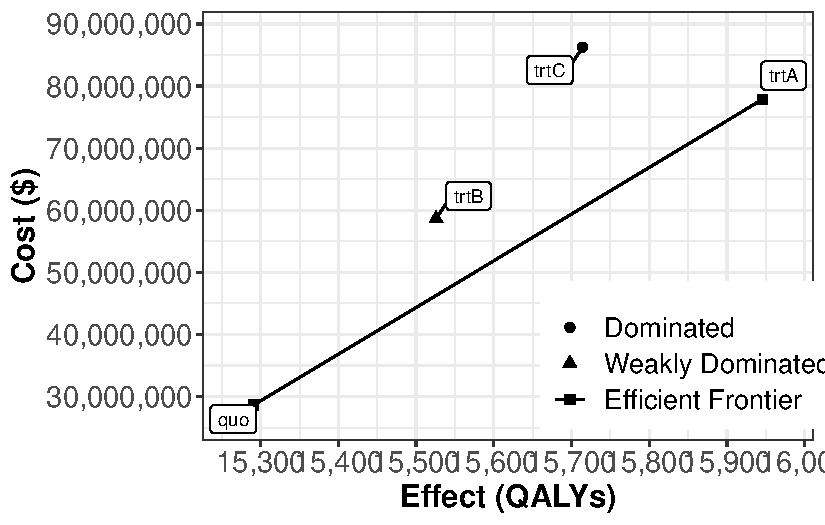
\includegraphics{MarkovDA_files/figure-pdf/cea-output-1.pdf}

}

\end{figure}

\hypertarget{step-7-one-way-sensitive-analysis}{%
\section{Step 7: One-way Sensitive
Analysis}\label{step-7-one-way-sensitive-analysis}}

Use owsa() function in the dampack package to create the one-way
sensitive analysis and tornado plot.

\begin{Shaded}
\begin{Highlighting}[]
\CommentTok{\# set lower \& upper case for cTrtA}
\CommentTok{\# params\_lower = params\_upper  = params\_sc}
\CommentTok{\# params\_lower$cTrtA = 8000}
\CommentTok{\# params\_upper$cTrtA = 10500}
\CommentTok{\# }
\CommentTok{\# result8000 = calculate\_icers(cost       = get\_ce(params\_lower)$cost,}
\CommentTok{\#                 effect     = get\_ce(params\_lower)$qaly,}
\CommentTok{\#                 strategies = v\_names\_str)}
\CommentTok{\# }
\CommentTok{\# result10500 = calculate\_icers(cost       = get\_ce(params\_upper)$cost,}
\CommentTok{\#                 effect     = get\_ce(params\_upper)$qaly,}
\CommentTok{\#                 strategies = v\_names\_str)}
\CommentTok{\# }
\CommentTok{\# \# set lower \& upper case for pStage3Death}
\CommentTok{\# params\_lower = params\_upper  = params\_sc}
\CommentTok{\# params\_lower$pStage3Death = 0.44}
\CommentTok{\# params\_upper$pStage3Death = 0.5}
\CommentTok{\# }
\CommentTok{\# calculate\_icers(cost       = get\_ce(params\_lower)$cost,}
\CommentTok{\#                 effect     = get\_ce(params\_lower)$qaly,}
\CommentTok{\#                 strategies = v\_names\_str)}
\CommentTok{\# }
\CommentTok{\# calculate\_icers(cost       = get\_ce(params\_upper)$cost,}
\CommentTok{\#                 effect     = get\_ce(params\_upper)$qaly,}
\CommentTok{\#                 strategies = v\_names\_str)}


\CommentTok{\#dampack\_dsa}

\NormalTok{simulate\_strategies }\OtherTok{=} \ControlFlowTok{function}\NormalTok{(params, }\AttributeTok{wtp =}\NormalTok{ params\_sc}\SpecialCharTok{$}\NormalTok{wtp) \{}
  \CommentTok{\# Create cost{-}effectiveness results data frame}
  \CommentTok{\# LY is the total dicounted life{-}years, here will not use. }
\NormalTok{  df\_ce }\OtherTok{\textless{}{-}} \FunctionTok{data.frame}\NormalTok{(}\AttributeTok{Strategy =}\NormalTok{ v\_names\_str,}
                      \AttributeTok{Cost =} \FunctionTok{numeric}\NormalTok{(n\_strategies),}
                      \AttributeTok{QALY =} \FunctionTok{numeric}\NormalTok{(n\_strategies),}
                      \AttributeTok{stringsAsFactors =} \ConstantTok{FALSE}\NormalTok{)}

\NormalTok{  result }\OtherTok{=} \FunctionTok{calculate\_icers}\NormalTok{(}\AttributeTok{cost =} \FunctionTok{get\_ce}\NormalTok{(}\AttributeTok{l\_m\_M =} \FunctionTok{build\_traces}\NormalTok{(params), }\AttributeTok{payoffs =} \FunctionTok{build\_payoffs}\NormalTok{(params), params)}\SpecialCharTok{$}\NormalTok{cost,}
                           \AttributeTok{effect =} \FunctionTok{get\_ce}\NormalTok{(}\AttributeTok{l\_m\_M =} \FunctionTok{build\_traces}\NormalTok{(params), }\AttributeTok{payoffs =} \FunctionTok{build\_payoffs}\NormalTok{(params), params)}\SpecialCharTok{$}\NormalTok{qaly,}
                           \AttributeTok{strategies =}\NormalTok{ v\_names\_str)}
  
\NormalTok{  df\_ce[}\FunctionTok{c}\NormalTok{(}\StringTok{"Cost"}\NormalTok{, }\StringTok{"QALY"}\NormalTok{,}\StringTok{"ICER"}\NormalTok{)] }\OtherTok{\textless{}{-}} \FunctionTok{c}\NormalTok{(result}\SpecialCharTok{$}\NormalTok{Cost,}
\NormalTok{                                result}\SpecialCharTok{$}\NormalTok{Effect,}
\NormalTok{                                result}\SpecialCharTok{$}\NormalTok{ICER)}
\NormalTok{  df\_ce[}\StringTok{"NMB"}\NormalTok{] }\OtherTok{\textless{}{-}}\NormalTok{ result}\SpecialCharTok{$}\NormalTok{Effect }\SpecialCharTok{*}\NormalTok{ wtp }\SpecialCharTok{{-}}\NormalTok{ result}\SpecialCharTok{$}\NormalTok{Cost}
  
  \FunctionTok{return}\NormalTok{(df\_ce)}
\NormalTok{\}}

\NormalTok{my\_owsa\_params\_range }\OtherTok{\textless{}{-}} \FunctionTok{data.frame}\NormalTok{(}\AttributeTok{pars =} \FunctionTok{c}\NormalTok{(}\StringTok{"cTrtA"}\NormalTok{, }\StringTok{"pStage3Death"}\NormalTok{),}
                                   \AttributeTok{min =} \FunctionTok{c}\NormalTok{(}\DecValTok{8000}\NormalTok{, }\FloatTok{0.3}\NormalTok{),}
                                   \AttributeTok{max =} \FunctionTok{c}\NormalTok{(}\DecValTok{10500}\NormalTok{, }\FloatTok{0.9}\NormalTok{))}

\NormalTok{l\_owsa\_det }\OtherTok{=} \FunctionTok{run\_owsa\_det}\NormalTok{(}\AttributeTok{params\_range =}\NormalTok{ my\_owsa\_params\_range,}
                           \AttributeTok{params\_basecase =}\NormalTok{ params\_sc,}
                           \AttributeTok{nsamp =} \DecValTok{2}\NormalTok{,}
                           \AttributeTok{FUN =}\NormalTok{ simulate\_strategies,}
                           \AttributeTok{outcomes =} \FunctionTok{c}\NormalTok{(}\StringTok{"Cost"}\NormalTok{, }\StringTok{"QALY"}\NormalTok{, }\StringTok{"ICER"}\NormalTok{, }\StringTok{"NMB"}\NormalTok{),}
                           \AttributeTok{strategies =}\NormalTok{ v\_names\_str,}
                           \AttributeTok{progress =} \ConstantTok{FALSE}\NormalTok{)}

\NormalTok{owsaNMBtrtA }\OtherTok{=}\NormalTok{ l\_owsa\_det}\SpecialCharTok{$}\NormalTok{owsa\_NMB[l\_owsa\_det}\SpecialCharTok{$}\NormalTok{owsa\_NMB[,}\StringTok{"strategy"}\NormalTok{] }\SpecialCharTok{==} \StringTok{"trtA"}\NormalTok{,]}
\NormalTok{owsaICERtrtA }\OtherTok{=}\NormalTok{ l\_owsa\_det}\SpecialCharTok{$}\NormalTok{owsa\_ICER[l\_owsa\_det}\SpecialCharTok{$}\NormalTok{owsa\_ICER[,}\StringTok{"strategy"}\NormalTok{] }\SpecialCharTok{==} \StringTok{"trtA"}\NormalTok{,]}
\FunctionTok{owsa\_tornado}\NormalTok{(owsaNMBtrtA)}
\end{Highlighting}
\end{Shaded}

\begin{figure}[H]

{\centering 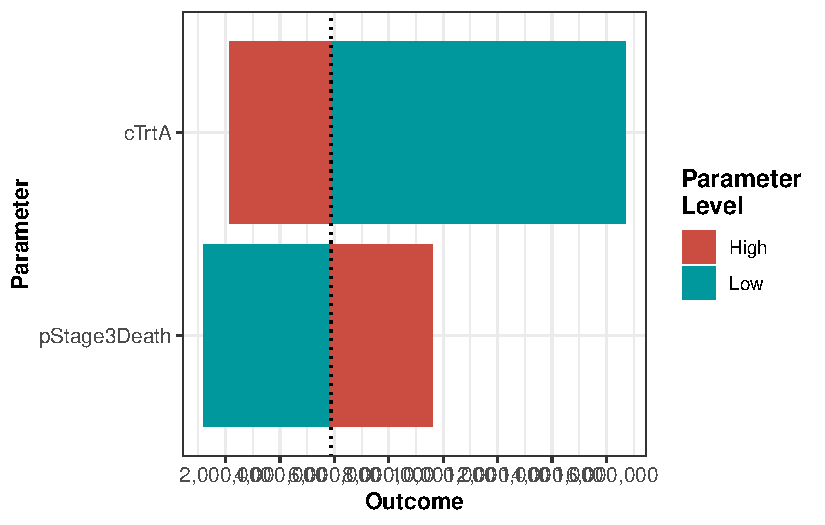
\includegraphics{MarkovDA_files/figure-pdf/owdsa-1.pdf}

}

\end{figure}

\begin{Shaded}
\begin{Highlighting}[]
\FunctionTok{owsa\_tornado}\NormalTok{(owsaICERtrtA)}
\end{Highlighting}
\end{Shaded}

\begin{figure}[H]

{\centering 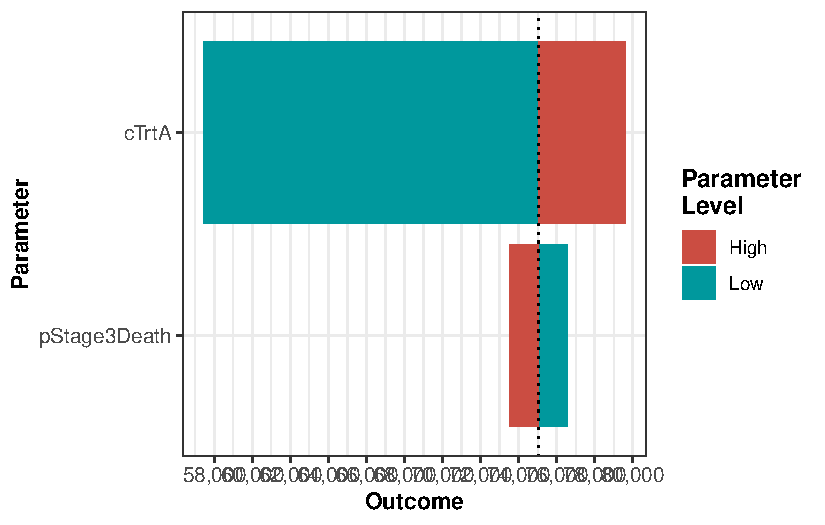
\includegraphics{MarkovDA_files/figure-pdf/owdsa-2.pdf}

}

\end{figure}

\begin{Shaded}
\begin{Highlighting}[]
\CommentTok{\# \# Select the net monetary benefit (NMB) owsa object}
\CommentTok{\# my\_owsa\_NMB \textless{}{-} l\_owsa\_det$owsa\_NMB}
\CommentTok{\# }
\CommentTok{\# \# Plot outcome of each strategy over each parameter range}
\CommentTok{\# plot(my\_owsa\_NMB,}
\CommentTok{\#      n\_x\_ticks = 4)}
\CommentTok{\# }
\CommentTok{\# owsa\_tornado(l\_owsa\_det$owsa\_NMB)}
\CommentTok{\# }
\CommentTok{\# owsa\_opt\_strat(l\_owsa\_det$owsa\_NMB)}
\end{Highlighting}
\end{Shaded}




\end{document}
